\section*{Exercice 142 -- Géométrie}
\setcounter{exo}{0}
%CCS PSI 2008


\begin{obj}
Respecter les normes de sécurité : l'effort de pincement doit être inférieur à \SI{150}{N}.
\end{obj}

Le système de verrouillage doit maintenir la porte fermée sous l’action des passagers et des
actions dues aux différences de pressions induites par le système de climatisation.
Un calcul préalable a établi que ces actions peuvent être modélisées par une
force $\vect{F}_{\text{basculateur}\rightarrow \text{bielle}}$ appliquée au point $E$, en position porte verrouillée. Le modèle du dispositif retenu est donné sur la figure suivante.

\begin{center}
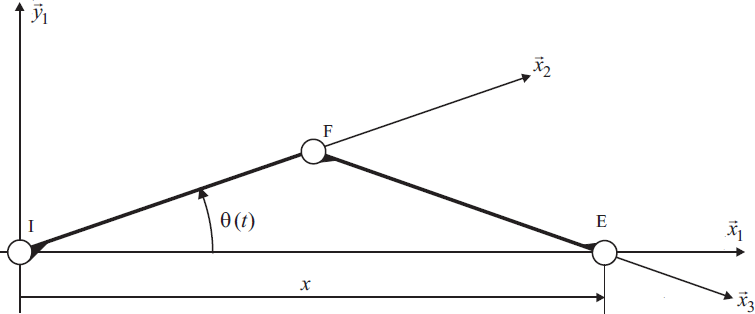
\includegraphics[width=\linewidth]{984_01}%
\end{center}

Soit le repère $\rep{1}\repere{I}{x_1}{y_1}{z_1}$ tel que $\vect{x_1}$ soit colinéaire à $\vect{IE}$ dans toutes
les configurations de la bielle de verrouillage $FE$ et du bras $IF$ lié au « stator »
du motoréducteur. Les notations retenues sont celles définies sur la figure 4, les
liaisons entre la bielle de verrouillage et le basculeur et entre le stator et la poutre
de fermeture sont respectivement une liaison pivot d’axe $\axe{E}{z_1}$ et une
liaison pivot d’axe $\axe{I}{z_1}$.
$\axe{I}{x_2}$ est lié au stator et tel que $\angl{x_1}{x_2}=\theta(t)$,
$\axe{F}{x_3}$ est lié à la bielle de verrouillage et tel que $\vect{x_3}$ soit colinéaire à $\vect{FE}$.
Pendant la phase de verrouillage, $\theta(t)$ varie quand le stator du moto réducteur
tourne par rapport à la poutre de fermeture. La vitesse angulaire sera notée
$\dot{\theta}(t)$, $\vect{IF}=\ell_1 \vect{x_2}$ et $\vect{FE}=\ell_2 \vect{x_3}$; par construction $\ell_1 \neq \ell_2$.

\subparagraph{}
\textit{Exprimer $x(t)$ en fonction de $\ell_1$, $\ell_2$ et $\theta(t)$ sous la forme
$x(t)=\lambda_1(t)\ell_1+\lambda_2(t)\ell_2$.}
\ifprof
\begin{corrige}
\end{corrige}
\else
\fi

\subparagraph{}
\textit{Exprimer la vitesse $\dot{x}$ du point $E$ appartenant au basculeur dans son mouvement
par rapport à $\rep{1}$ en fonction de $\ell_1$, $\ell_2$, $\theta(t)$ et $\dot{\theta}(t)$ sous la forme $A(\theta)\dot{x}=B(\theta)\dot{\theta}$.}
\ifprof
\begin{corrige}
\end{corrige}
\else
\fi

\subparagraph{}
\textit{Montrer qu’il existe une valeur de pour laquelle le basculeur ne pourra fournir aucune puissance au système. Expliquer pourquoi cette position est instable.}
\ifprof
\begin{corrige}
\end{corrige}
\else
\fi

\subparagraph{}
\textit{Un tel mécanisme est appelé mécanisme à genouillère. Existe-t-il dans le
système de fermeture d’autres cas d’utilisation de ce principe ? Dans l’affirmative,
indiquer pour chacun, les trois points considérés et le mouvement qui est
bloqué.}
\ifprof
\begin{corrige}
\end{corrige}
\else
\fi

\subparagraph{}
\textit{Expliquer quelle est la fonction des butées 1 et 2 (figures suivantes) et préciser
en la justifiant, leur position de réglage ?}
\ifprof
\begin{corrige}
\end{corrige}
\else
\fi

\subparagraph{}
\textit{Expliquer la pertinence de cette solution à empêcher l’ouverture des vantaux
quelle que soit la poussée des passagers. Conclure quant à la satisfaction de l'exigence.}
\ifprof
\begin{corrige}
\end{corrige}
\else
\fi


\begin{center}
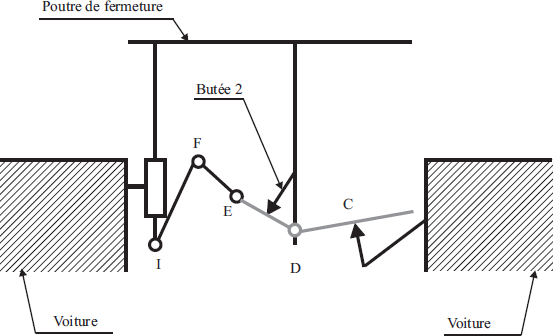
\includegraphics[width=\linewidth]{984_02}%

 \textit{Étape de coulissement}
\end{center}

\begin{center}
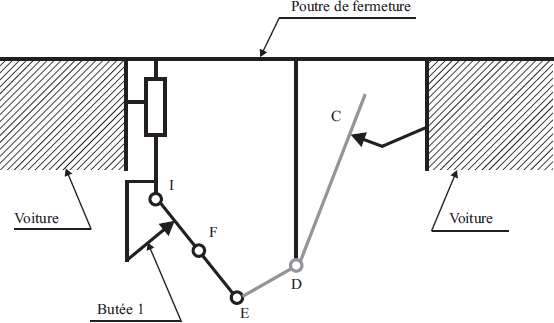
\includegraphics[width=\linewidth]{984_03}%

 \textit{Étape verrouillée}
\end{center}


\begin{enumerate}
\item $x(t)=\ell_1 \cos\theta +\ell_2 \sqrt{1-r^2\sin^2\theta}$.
\item $A=\sqrt{1-r^2\sin^2\theta}$, $B=-\ell_1\sin\theta\sqrt{1-r^2\in^2\theta}-\ell_2r^2\sin\theta\cos\theta$.
\item $\theta=0\degres$.
\item ...
\item ...
\end{enumerate}
